\documentclass[journal]{IEEEtran}
\usepackage[a5paper, margin=10mm]{geometry}
%\usepackage{lmodern} % Ensure lmodern is loaded for pdflatex
\usepackage{tfrupee} % Include tfrupee package

%iffalse
\let\negmedspace\undefined
\let\negthickspace\undefined
\usepackage{gvv-book}
\usepackage{gvv}
\usepackage{cite}
\usepackage{amsmath,amssymb,amsfonts,amsthm}
\usepackage{algorithmic}
\usepackage{graphicx}
\usepackage{textcomp}
\usepackage{xcolor}
\usepackage{txfonts}
\usepackage{listings}
\usepackage{enumitem}
\usepackage{mathtools}
\usepackage{gensymb}
\usepackage{comment}
\usepackage[breaklinks=true]{hyperref}
\usepackage{tkz-euclide} 
\usepackage{listings}                                        
%\def\inputGnumericTable{}                                 
\usepackage[latin1]{inputenc}                                
\usepackage{color}                                            
\usepackage{array}                                            
\usepackage{longtable}                                       
\usepackage{calc}                                             
\usepackage{multirow}                                         
\usepackage{hhline}                                           
\usepackage{ifthen}                                           
\usepackage{lscape}
\usepackage{tabularx}
\usepackage{array}
\usepackage{float}
\usepackage{multicol}

\newcommand{\BEQA}{\begin{eqnarray}}
\newcommand{\EEQA}{\end{eqnarray}}
%\newcommand{\define}{\stackrel{\triangle}{=}}

\setlength{\headheight}{1cm} % Set the height of the header box
\setlength{\headsep}{0mm}     % Set the distance between the header box and the top of the text


%\usepackage[a5paper, top=10mm, bottom=10mm, left=10mm, right=10mm]{geometry}


\setlength{\intextsep}{10pt} % Space between text and floats

% Marks the beginning of the document
\begin{document}
\onecolumn
\bibliographystyle{IEEEtran}
\vspace{3cm}

%\renewcommand{\theequation}{\theenumi}
\numberwithin{equation}{enumi}
\numberwithin{figure}{enumi}
\renewcommand{\thefigure}{\theenumi}
\renewcommand{\thetable}{\theenumi}

\title{1-1.11-3}
\author{ai24btech11030 - Shiven Bajpai}
\maketitle

\renewcommand{\thefigure}{\theenumi}
\renewcommand{\thetable}{\theenumi}

\textbf{Question: } If a line makes 60\degree  and 45\degree  angles with the positive directions of the X-axis and Z-axis respectively, then find the angle that it makes with the positive direction of the Y-axis. Hence, write the direction cosines of the line. 
\\

\textbf{Solution: } Let $\alpha,\; \beta$ and $\gamma$ be the angles made by the line with the X, Y and Z axes respectively. Now the unit direction vector $\vec{x}$ can be expressed as

\begin{align*}
	\vec{x} &= \myvec{\cos\alpha\\\cos\beta\\\cos\gamma}\\
	\Vert\vec{x}\Vert &= 1\\
	\\
	\sqrt{\vec{x}\vec{x}^\text{T}} &= 1\\
	\cos^2\alpha + \cos^2\beta + \cos^2\gamma &= 1\\
	\cos^260\degree + \cos^2\beta + \cos^245\degree &= 1\\
	\frac{1}{4} + \cos^2\beta + \frac{1}{2} &= 1\\
	\cos^2\beta &= \frac{1}{4}\\
	\cos\beta &= \pm\frac{1}{2}\\
	\beta &= 60\degree\\
\end{align*}

Hence the direction cosines are

$$\vec{x} = \myvec{\cos\alpha\\\cos\beta\\\cos\gamma} = \myvec{\cos60\degree\\\cos60\degree\\\cos45\degree} = \myvec{\frac{1}{2}\\\frac{1}{2}\\\frac{1}{\sqrt{2}}}$$

\newpage

\begin{figure}[H]
	\centering
	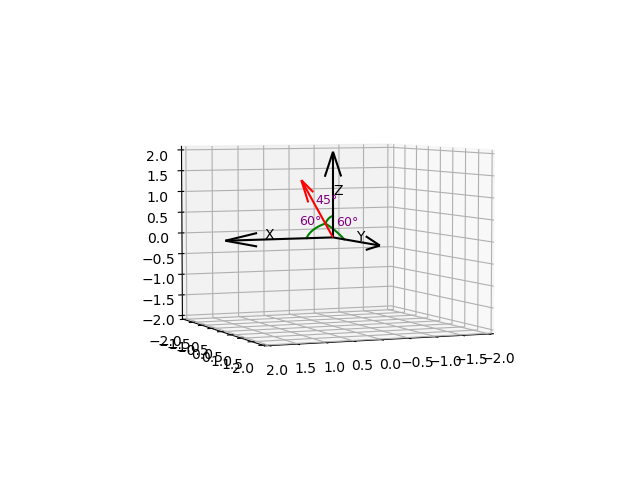
\includegraphics[width=0.75\columnwidth]{Figures/Figure.png}
	\caption{Plot of the described vector}
	\label{fig}
\end{figure}

Code for this plot can be found at:
\begin{lstlisting}
    Codes/main.py
    Codes/main.c
\end{lstlisting}

\end{document}
